\documentclass{beamer}

\usepackage[utf8]{inputenc}
\usepackage{amsmath}
\usetheme{Madrid}% modern fork of the metropolis theme
\usepackage{booktabs}
\usepackage{float}

\definecolor{mPurple}{RGB}{91,48,105}
\setbeamercolor{palette primary}{bg=mPurple}
\setbeamercolor{normal text}{fg=black}



\title{Stress Testing en Sistemas de Pensiones}
\subtitle{Módulo 1: Fundamentos}
\author{Francisco A. Ramírez \\ 
MACROPOL- Macroeconomía y Economía Pública}
\date{}

\begin{document}

\frame{\titlepage}
\begin{frame}{Contenido}
\tableofcontents    
\end{frame}

\section{1. Introducción}
%--------------------------------------
\subsection{1.1. Descripción del curso}
\begin{frame}[t]{Descripción del curso}

\begin{itemize}

    \item Los sistemas de pensiones enfrentan riesgos crecientes derivados de la interacción entre la macroeconomía, el mercado financiero y la demografía: inflación, desempleo, tasas de interés, o aumentos en la longevidad pueden comprometer la sostenibilidad y suficiencia de las pensiones.
\vspace{0.4cm} 
    \item El \textit{stress testing} se ha consolidado como una herramienta clave para la gestión de riesgos y la supervisión macroprudencial.
\vspace{0.4cm}
    \item Este curso propone un enfoque integrado que adapta metodologías utilizadas en banca y regulación financiera al análisis de sistemas de pensiones, incorporando simultáneamente dimensiones macroeconómicas, financieras y actuariales.

\end{itemize}

    
\end{frame}
%---------------------------------------
\subsection{1.2. Objetivo general}
\begin{frame}[t]{Objetivo general}
\vspace{0.4cm}
    \begin{itemize}
    
        \item Desarrollar en los participantes las competencias necesarias para:
        
        \begin{itemize}
            \item diseñar, 
            \item implementar e
            \item interpretar
        \end{itemize} 
        ejercicios de \textit{stress testing} aplicados a sistemas de pensiones de capitalización individual, integrando riesgos macroeconómicos, financieros y actuariales, con el fin de evaluar la resiliencia del sistema previsional y apoyar la toma de decisiones regulatorias y de política pública.
    \end{itemize}
\end{frame}
%---------------------------------------
\subsection{1.3. Objetivos específicos}
\begin{frame}[t]{Objetivos específicos}
\begin{itemize}
    \item Comprender el marco conceptual del \textit{stress testing}
    \item Identificar y medir riesgos previsionales clave
    \item Evaluar el impacto de shocks sobre portafolios previsionales
    \item Incorporar riesgos actuariales en el análisis
    \item Integrar resultados en un marco de stress testing sistémico
    \item Traducir resultados en implicaciones para las políticas públicas
\end{itemize}
    
\end{frame}
%--------------------------------------
\subsection{1.4. Estructura del curso}
\begin{frame}{Estructura del curso}

\footnotesize
\begin{tabular}{p{0.2cm} p{4cm} p{1cm} p{4cm}}
\hline
\textbf{M} & \textbf{Módulo} & \textbf{Horas} & \textbf{Contenidos Clave} \\
\hline

1 & Fundamentos de Stress Testing & 4h & Concepto, marco de riesgo previsional, baseline vs adverso \\

2 & Riesgos Previsionales & 5h & Mercado, longevidad, liquidez, indicadores de vulnerabilidad \\

3 & Escenarios Macro-Financieros & 6h & VAR, ARIMA, Monte Carlo, diseño de escenarios \\

4 & Stress Testing del Portafolio & 5h & Modelos multifactoriales, GARCH, sensibilidad a shocks \\

5 & Stress Testing Actuarial & 5h & Longevidad, proyección de pensiones, tasa de reemplazo \\

6 & Integración y Reporte & 5h & Stress testing integral, interpretación, política pública \\

\hline
\end{tabular}

\vspace{0.3cm}

\textit{Enfoque integrado: macroeconomía, finanzas y actuarial aplicado a sistemas previsionales}


\end{frame}
%--------------------------------------
\subsection{1.5 Calendario de clases}
\begin{frame}{Calendario de clases}
\footnotesize
\begin{table}[H]
\centering
\begin{tabular}{c c c l}
\toprule
\textbf{Sesión} & \textbf{Fecha} & \textbf{Modalidad} & \textbf{Comentario} \\
\midrule
1  & 22-abr-2026 & Virtual     & Inicio del curso \\
2  & 24-abr-2026 & Virtual     &  \\
3  & 28-abr-2026 & Virtual     &  \\
4  & 30-abr-2026 & Virtual     &  \\
5  & 04-may-2026 & Virtual     &  \\
6  & 06-may-2026 & Presencial  & Primera sesión presencial \\
7  & 08-may-2026 & Virtual     &  \\
8  & 13-may-2026 & Virtual     &  \\
9  & 15-may-2026 & Virtual     &  \\
10 & 20-may-2026 & Virtual     &  \\
11 & 22-may-2026 & Presencial  & Segunda sesión presencial \\
12 & 27-may-2026 & Virtual     &  \\
13 & 29-may-2026 & Virtual     &  \\
14 & 03-jun-2026 & Virtual     &  \\
15 & 10-jun-2026 & Presencial  & Cierre del curso \\
\bottomrule
\end{tabular}
\end{table}
\end{frame}
%--------------------------------------
\subsection{1.6 Metodología de trabajo}
\begin{frame}{Metodología de trabajo}
El curso combina:
\begin{itemize}
    \item Macroeconomía (escenarios)
    \item Finanzas (portafolio)
    \item Actuarial (beneficios)
    \item Simulación (Monte Carlo)
\end{itemize}
\vspace{0.4cm}

El curso utiliza cuatro bloques de datos:

\begin{itemize}
\item Macroeconómicos: PIB, inflación, tasas, retornos
\item Financieros: portfolios, volatilidad, correlaciones
\item Afiliados: edad, salario, saldo
\item Actuariales: mortalidad, edad de retiro
\end{itemize}

\end{frame}
%-----------------------------------------
\begin{frame}{Metodología de trabajo}

El curso utilizar:
\begin{itemize}
    \item \textbf{R} como lenguaje principal
    \item Paquetes:
    \begin{itemize}
        \item \texttt{vars} (escenarios macro)
        \item \texttt{rugarch} (volatilidad)
        \item \texttt{tidyverse} (manejo de datos)
    \end{itemize}
\end{itemize}

El estudiante desarrollará:

\begin{itemize}
    \item Construcción de escenarios macro
    \item Modelación de retornos
    \item Simulación de trayectorias individuales
    \item Cálculo de pensiones
\end{itemize}

\vspace{0.5cm}
\textbf{Producto final:} stress test completo del sistema.

  
\end{frame}
%-----------------------------------------
\begin{frame}[t]{Metodología de trabajo}
\textbf{Evaluación}
\begin{itemize}
    \item Ejercicios prácticos por módulo
    \item Talleres en R
    \item Proyecto final integrador
\end{itemize}

\vspace{0.5cm}
\textbf{Criterios de evalaución:}

\begin{itemize}
    \item Coherencia económica del escenario
    \item Correcta implementación técnica
    \item Interpretación de resultados
\end{itemize}
  
\end{frame}
%-----------------------------------------
\subsection{1.7 Base de datos}
\begin{frame}[t]{Base de datos del curso}
Se construirá una base integrada:

\begin{itemize}
\item Series macroeconómicas
\item Retornos de activos
\item Datos simulados de afiliados
\end{itemize}

\vspace{0.5cm}
La base simulada representa un sistema previsional simplificado. 

\vspace{0.5cm}
\textbf{Uso:} La base de datos será un insumo para todos los ejercicios del curso.

\vspace{0.3cm}
Con ella simulamos la cadena:

\centering
\textbf{Escenario → Retornos → Aportes → Saldo → Pensión}
\end{frame}

%-----------------------------------------
\begin{frame}[t]{Estructura de la base}
La base se organiza en tres bloques:

\begin{itemize}
\item Datos macroeconómicos
\item Datos financieros
\item Datos de afiliados
\end{itemize}

\vspace{0.5cm}
\textbf{Enfoque:} integración de riesgos
\end{frame}

\section{2. Módulo 1: Fundamentos de Stress Testing en Pensiones}
% Slide 2
\begin{frame}[t]{Objetivo del módulo}
\begin{itemize}
\item Comprender qué es el \textit{stress testing} o prueba de estrés.
\item Entender su relevancia en sistemas de pensiones
\item Diferenciar su aplicación respecto al sector bancario
\end{itemize}
\end{frame}

% Slide 3
\begin{frame}[t]{Contexto económico}

\begin{itemize}
    \item Crisis Financiera Global trajo la atención a las pruebas de estrés de instituciones financieras.
    \vspace{0.3cm}
    \item La crisis dej\'o expuesta las fallas en medici\'on de riesgos y subestimaci\'on de eventos extremos.
    \vspace{0.3cm}
    \item Tambi\'en se gener\'o la necesidad de enfoques integrales y prospectivos (forward-looking).
    \vspace{0.3cm}
    \item El \textit{stress testing} se consolidad como una herramienta central de la gesti\'on de riesgos.
\end{itemize}

\end{frame}
%-----------------------------------------------------
\begin{frame}[t]{¿Qué es el \textit{stress testing?}}
\textbf{Definiciones:}
\begin{itemize}

    \item Es un escenario \textit{"What if..."}.
    \vspace{0.3cm}
    \item Mide la sensibilidad de un portafolio, una institución, o un sistema financiero a shocks excepcionales pero plausibles.
    \vspace{0.3cm}
    \item Evaluación de la resiliencia de un sistema ante escenarios extremos pero plausibles.
    \vspace{0.3cm}
    \item Consiste en evaluar el impacto de escenarios extremos, pero plausibles,  que no son considerados por el VaR o el ES, pues estos auque útiles, son retrospectivos. La gestion de riesgos concierne a lo que puede pasar en el futuro.
\end{itemize}

\end{frame}
%-----------------------------------------------------
\begin{frame}[t]{¿Qué es el \textit{stress testing?}}
\textbf{Intuición económica:}
\begin{itemize}
\item No modela el promedio
\item Se enfoca en eventos extremos
\item Evalúa riesgo sistémico
\item Qu\'e se necesita para "quebrar" una instituci\'on o un sistema financiero.
\end{itemize}
\end{frame}
%-----------------------------------------
\begin{frame}{¿Por qué es necesario el Stress Testing?}

\begin{itemize}

\item \textbf{Anticipación de vulnerabilidades:}  
Permite evaluar el impacto de escenarios extremos pero plausibles (caídas de mercado, shocks de tasas de interés, aumentos en la longevidad) sobre la sostenibilidad del sistema previsional.

\vspace{0.5cm}

\item \textbf{Soporte a la regulación y política pública:}  
Facilita la identificación de riesgos sistémicos y el diseño de medidas preventivas para proteger los ahorros previsionales y garantizar la estabilidad del sistema.

\end{itemize}

\end{frame}
%---------------------------------------
\begin{frame}{¿Qué instituciones utilizan Stress Testing?}

\begin{itemize}

\item \textbf{Bancos centrales y supervisores financieros:}  
Evaluar la estabilidad del sistema financiero y detectar riesgos sistémicos (enfoque macroprudencial).

\vspace{0.3cm}

\item \textbf{Administradoras de fondos de pensiones (AFP):}  
Medir el impacto de shocks en los portafolios y en las tasas de reemplazo de los afiliados.

\vspace{0.3cm}

\item \textbf{Bancos y entidades financieras:}  
Gestionar riesgos de mercado, crédito y liquidez, y cumplir con requerimientos regulatorios (Basilea).

\vspace{0.3cm}

\item \textbf{Organismos internacionales (FMI, Banco Mundial):}  
Realizar evaluaciones de estabilidad financiera (FSAP) y análisis comparativos entre países.

\vspace{0.3cm}

\item \textbf{Ministerios de Hacienda y reguladores previsionales:}  
Evaluar la sostenibilidad fiscal y los riesgos del sistema de pensiones.

\end{itemize}

\end{frame}
%---------------------------------------
\begin{frame}{¿Cuándo el Stress Testing es informativo?}

\begin{itemize}

\item \textbf{Integra múltiples fuentes de riesgo:}  
Considera de manera conjunta riesgos de mercado, crédito, liquidez y demográficos, evitando una visión parcial del sistema.

\vspace{0.3cm}

\item \textbf{Captura los principales drivers de riesgo:}  
Identifica y modela las variables clave (tasas de interés, retornos, inflación, longevidad) que determinan los resultados previsionales.

\vspace{0.3cm}

\item \textbf{Se basa en escenarios económicamente coherentes:}  
Los shocks deben responder a una narrativa macro-financiera consistente (baseline vs adverso).

\vspace{0.3cm}

\item \textbf{Permite traducir shocks en métricas relevantes:}  
Impacta variables clave como valor del portafolio, densidad de cotización y tasa de reemplazo.

\vspace{0.3cm}

\item \textbf{Es útil para la toma de decisiones:}  
Sus resultados informan políticas de inversión, regulación y gestión del riesgo previsional.

\end{itemize}

\end{frame}
%-----------------------------------------------
\begin{frame}{Tipos de Stress Tests}
\begin{itemize}

    \item \textbf{Análisis de sensibilidad}: es un proceso de determinar c\'omo cambios en un factor de riesgo (par\'ametro) impacta\'a una instituci\'on o portfolio. \textit{Por ejemplo, un cambio de 200pb en la tasa de inter\'es sobre un portfolio}.
\vspace{0.3cm}
    \item \textbf{An\'alisis de escenario}: estudia el efecto de un movimiento simult\'aneo en un grupo de factores de riesgo, analizando la respuesta del portfolio a un escenario completo.
\end{itemize}
\centering
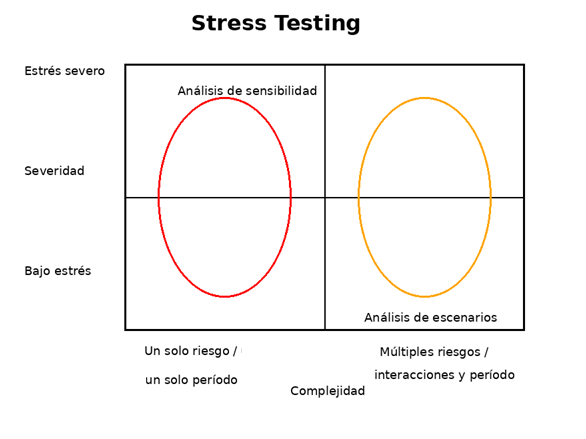
\includegraphics[width=0.7\textwidth]{fig-1-stress-testing.png}
    
\end{frame}
%----------------------------------------------
\begin{frame}{M\'etodos de Stress Testing}
\begin{itemize}

    \item \textbf{Hist\'orico versus hipot\'etico}
    
    \begin{itemize}
    
        \item \textbf{Escenario hist\'orico}: basado en eventos del pasado. \textit{Por ejemplo, crisis de deuda en los mercados emergentes de la d\'ecada de los 90's}. Son \'utiles cuando algun aspecto del escenario hsit\'orico se espera que reocurra. Estos escenarios son retrospectivos y pierden relevancia en el tiempo.
     
        \vspace{0.3cm}
    
        \item \textbf{Escenario hipot\'etico}: considera desarrollos plausibles en el futuro.
     \end{itemize}
     
    \item \textbf{Determin\'istico verus Estoc\'astico}

    \begin{itemize}
    
        \item \textbf{Determin\'isticos}: est\'an definidos a priori sin alguna referencia a su verosimilitud.

        \vspace{0.3cm}
        
        \item \textbf{Estoc\'asticos}: son escenarios generados para producir una distribuci\'o de resultados sobre la base de supuestos de las distribuciones subyacentes.    
    \end{itemize}
\end{itemize}
\end{frame}
%----------------------------------------------
\begin{frame}{Stress Testing reverso}
\begin{itemize}

    \item El enfoque tradicional al \textit{stress} testing define el deterioro en los factores de riesgo, y entonces eval\'ua el impacto de esos cambios en el portfolio. Por ejemplo: \[
\uparrow \text{FFR} \Rightarrow \uparrow \text{Yield bonos del gobierno}
\]

\item \textbf{stress testing Reverso}: usando para evaluar la resiliencia  de un portfolio a eventos extremos v\'ia identificar cuales eventos pueden conducir a p\'erdidas que excedan un nivel dado. Por ejemplo, el proceso ser\'ia as\'i:

    
\end{itemize}
\[\text{p\'erdida  del portafolio} \Rightarrow\ \text{identificar eventos }\]
\end{frame}

%----------------------------------------------
\begin{frame}{Enfoques para la elaboración de Stress Testing}

\begin{itemize}

\item \textbf{Enfoque contable (balance sheet approach):}  
Evalúa el impacto de escenarios sobre los estados financieros, proyectando activos, pasivos y capital bajo distintos shocks.

\vspace{0.3cm}

\item \textbf{Enfoque basado en precios de mercado:}  
Utiliza información de mercado (precios de activos, spreads, volatilidad) para inferir pérdidas y riesgos en tiempo real.

\vspace{0.3cm}

\item \textbf{Enfoque macro-financiero:}  
Vincula variables macroeconómicas (PIB, inflación, tasas de interés) con variables financieras mediante modelos econométricos (VAR, ARIMA).

\vspace{0.3cm}

\item \textbf{Enfoque integrado (mejor práctica):}  
Combina los tres enfoques para capturar interacciones entre economía real, mercados financieros y balances previsionales.

\end{itemize}

\end{frame}
%---------------------------------------------
\begin{frame}{Stress Testing en sistemas de pensiones}

\begin{itemize}

\item \textbf{Tipos de planes de pensión:}  
\begin{itemize}
    \item Beneficio definido (BD): riesgo asumido por el patrocinador  
    \item Contribución definida (CD): riesgo asumido por el afiliado  
    \item Sistemas mixtos: combinación de ambos esquemas
\end{itemize}

\vspace{0.3cm}

\item \textbf{Dimensiones clave del Stress Testing:}  
\begin{itemize}
    \item \textbf{Riesgo de mercado:} impacto en retornos y valor del portafolio  
    \item \textbf{Riesgo de longevidad:} aumento en la esperanza de vida  
    \item \textbf{Riesgo macroeconómico:} inflación, tasas de interés, crecimiento  
    \item \textbf{Resultados previsionales:} tasa de reemplazo y suficiencia de pensiones
\end{itemize}

\end{itemize}

\end{frame}
%---------------------------------------------
\begin{frame}[t]{Stress Testing: Banca vs Pensiones}
\begin{tabular}{|l|l|l|}
\hline
\textbf{Aspecto} & \textbf{Banca} & \textbf{Pensiones} \\
\hline
Horizonte & Corto & Largo \\
Riesgo clave & Solvencia & Adecuación \\
Variable objetivo & Capital & Tasa de reemplazo \\
Enfoque & Balance & Ciclo de vida \\
\hline
\end{tabular}
\end{frame}
%---------------------------------------------
\begin{frame}{Stress Testing  sistemas de pensiones en diferentes pa\'ises}
\footnotesize
\begin{table}[H]
\centering

\begin{tabular}{|l|l|p{6cm}|}
\hline
\textbf{País} & \textbf{Tipo} & \textbf{Tipo de pruebas de estrés} \\
\hline
Chile & CD & Retorno mínimo, VaR \\
\hline
Rep. Checa & Híbrido & Escenarios base con variables macroeconómicas \\
\hline
Alemania & BD & Prueba de estrés con cuatro escenarios: solo bonos, solo acciones, bonos y acciones, acciones y propiedades \\
\hline
Islandia & BD & Ratio de financiamiento frente a un conjunto de 10 variables críticas \\
\hline
Israel & CD & Identificación de las principales fuentes de riesgo de mercado: tasa de interés, spread, mercado accionario y tipo de cambio \\
\hline
México & CD & VaR \\
\hline
Noruega & BD & Análisis de alerta temprana y pruebas sobre riesgo de mercado, riesgo de seguros, riesgo de contraparte y riesgo operacional \\
\hline
\end{tabular}

\vspace{0.3cm}
\footnotesize{Fuente: Encuesta de la IOPS, respuestas de autoridades supervisoras.}
\end{table}
    
\end{frame}
%---------------------------------------------
% Slide 6
\begin{frame}{Sistema de capitalización individual}
Depende de:
\begin{itemize}
\item Aportes
\item Retornos financieros
\item Longevidad
\end{itemize}

\vspace{0.5cm}

\textbf{Conclusión:} Sistema altamente sensible al ciclo económico.
\end{frame}
%---------------------------------------
\begin{frame}{Gobernanza y requerimientos de supervisi\'on para el Stress Test}
\begin{itemize}
    \item Como herramienta de gesti\'on de riesgos el stress test depende de:
    \begin{itemize}
        \item gobernanza robusta
        \item metodolog\'ia transparente y s\'olida
        \item reporte efectivo de los resultados 
    \end{itemize}
    \item La metodolog\'ia tiene que ser revisada y actualizada con frecuencia.
    \item Por su complejidad, quien administra la prueba debe depender de un comit\'e  de riesgo, que diseñe, ejecute y revise la prueba de estr\'es.
    
\end{itemize}
    
\end{frame}

%----------------------------------------
\begin{frame}{Elecciones fundamentales en el diseño de un Stress Test}

\begin{itemize}

\item \textbf{Definición del universo de riesgos:}  
Identificación de los riesgos relevantes (mercado, crédito, liquidez, longevidad, macroeconómico).

\vspace{0.3cm}

\item \textbf{Alcance del ejercicio:}  
Selección de instituciones, horizonte temporal del escenario y magnitud de los shocks (baseline vs adverso).

\vspace{0.3cm}

\item \textbf{Modelo de transmisión:}  
Construcción de modelos que traduzcan shocks macro-financieros en impactos sobre variables clave (portafolio, balances, pensiones).

\vspace{0.3cm}

\item \textbf{Criterios de evaluación:}  
Definición de métricas y umbrales para determinar resiliencia (ej. solvencia, pérdidas, tasa de reemplazo).

\vspace{0.3cm}

\item \textbf{Estrategia de comunicación:}  
Decisión sobre el nivel de divulgación de resultados y su uso en supervisión y política pública.

\end{itemize}

\end{frame}
%----------------------------------------------------
\begin{frame}{Mejores pr\'acticas en Stress Testing, Viñals (2012)}
\begin{itemize}
    \item Definir el per\'imetro institucional para el test.
    \item Identificar los canales relevantes para la propagaci\'on de riesgos.
    \item Incluir todos los riesgos y buffers materiales.
    \item Usar el punto de vista del inversionista en el diseño del stress test.
    \item Enfocarse en los riesgos de cola.
    \item Resaltar lo estrat\'egico en la comunicaci\'on de resultados.
    \item Atenci\'on con los "cisnes negros".
\end{itemize}
    
\end{frame}

%------------------------------------------------
\begin{frame}{Enfoque Regulatorio}
\textbf{Contexto}
\begin{itemize}
\item El stress testing surge como herramienta de supervisión financiera
\item En pensiones, su adopción es más reciente y heterogénea
\end{itemize}

\textbf{Intuición económica}
\begin{block}{}
El regulador busca evaluar la resiliencia del sistema previsional ante shocks extremos
\end{block}

\textbf{Interpretación}
\begin{itemize}
\item No es solo gestión de riesgo: es instrumento de política pública
\end{itemize}
\end{frame}

%------------------------------------------------
\begin{frame}{Objetivos del Regulador}
\textbf{Tres objetivos principales}
\begin{enumerate}
\item Protección del afiliado
\item Estabilidad financiera
\item Sostenibilidad del sistema
\end{enumerate}

\textbf{Trade-off clave}
\begin{block}{}
Mayor seguridad $\leftrightarrow$ menor rentabilidad esperada
\end{block}

\textbf{Interpretación}
\begin{itemize}
\item El diseño del stress test refleja este trade-off
\end{itemize}
\end{frame}

%------------------------------------------------
\begin{frame}{Tipología de Enfoques}
\textbf{Clasificación principal}
\begin{itemize}
\item Microprudencial
\item Macroprudencial
\item Híbrido
\end{itemize}

\textbf{Modelo conceptual}
\[
ST = f(\text{nivel de análisis}, \text{riesgos}, \text{horizonte})
\]

\textbf{Interpretación}
\begin{itemize}
\item La elección depende del rol del regulador
\end{itemize}
\end{frame}

%------------------------------------------------
\begin{frame}{Enfoque Microprudencial}
\textbf{Contexto}
\begin{itemize}
\item Evaluación a nivel de fondo o AFP
\end{itemize}

\textbf{Variables clave}
\begin{itemize}
\item Valor del portafolio
\item Rentabilidad
\item Riesgo de mercado
\end{itemize}

\textbf{Modelo}
\[
V^{stress} = V (1 + r_{stress})
\]

\textbf{Interpretación}
\begin{itemize}
\item Foco en solvencia y pérdidas individuales
\end{itemize}
\end{frame}

%------------------------------------------------
\begin{frame}{Enfoque Macroprudencial}
\textbf{Contexto}
\begin{itemize}
\item Evaluación del sistema previsional completo
\end{itemize}

\textbf{Variables clave}
\begin{itemize}
\item Tasa de reemplazo
\item Sostenibilidad fiscal
\item Cobertura del sistema
\end{itemize}

\textbf{Modelo}
\[
TR = \frac{\text{Pensión}}{\text{Salario}}
\]

\textbf{Interpretación}
\begin{itemize}
\item Foco en bienestar agregado
\end{itemize}
\end{frame}

%------------------------------------------------
\begin{frame}{Enfoque Híbrido}
\textbf{Contexto}
\begin{itemize}
\item Integra micro y macro
\end{itemize}

\textbf{Modelo}
\[
Pensión = f(\text{retornos}, \text{contribuciones}, \text{longevidad})
\]

\textbf{Interpretación}
\begin{itemize}
\item Permite conectar mercado con resultados previsionales
\end{itemize}

\textbf{Insight}
\begin{block}{}
Es el enfoque más consistente con política pública moderna
\end{block}
\end{frame}

%------------------------------------------------
\begin{frame}{Horizonte del Stress Testing}
\textbf{Dos enfoques}
\begin{itemize}
\item Corto plazo (mark-to-market)
\item Largo plazo (ciclo de vida)
\end{itemize}

\textbf{Trade-off}
\begin{block}{}
Precisión financiera vs relevancia previsional
\end{block}

\textbf{Interpretación}
\begin{itemize}
\item Pensiones requieren horizonte largo
\end{itemize}
\end{frame}

%------------------------------------------------
\begin{frame}{Tipos de Riesgos Cubiertos}
\textbf{Clasificación}
\begin{itemize}
\item Riesgo de mercado
\item Riesgo de longevidad
\item Riesgo de inflación
\item Riesgo de contribuciones
\end{itemize}

\textbf{Modelo}
\[
Riesgo_{total} = \sum_i Riesgo_i
\]

\textbf{Interpretación}
\begin{itemize}
\item En pensiones, el riesgo actuarial es tan importante como el financiero
\end{itemize}
\end{frame}


%------------------------------------------------
\begin{frame}{Uso Regulatorio}
\textbf{Aplicaciones}
\begin{itemize}
\item Supervisión de fondos
\item Diseño de regulación
\item Comunicación de riesgos
\end{itemize}

\textbf{Interpretación}
\begin{itemize}
\item El stress test guía decisiones regulatorias
\end{itemize}
\end{frame}

%------------------------------------------------
\begin{frame}{Lecciones Clave}
\textbf{Resultados}
\begin{itemize}
\item No hay enfoque único
\item El diseño depende del sistema
\item La variable objetivo es crítica
\end{itemize}

\textbf{Modelo}
\[
Diseño = f(\text{objetivo}, \text{sistema}, \text{riesgos})
\]

\textbf{Interpretación}
\begin{itemize}
\item El regulador define qué riesgo importa
\end{itemize}
\end{frame}


%------------------------------------------------
\begin{frame}{Experiencia internacional}

\begin{itemize}
\item El stress testing en pensiones es más reciente que en banca.
\vspace{0.2cm}
\item Alta heterogeneidad institucional
\vspace{0.2cm}
\item No existe un modelo único: cada país refleja prioridades regulatorias distintas
\vspace{0.2cm}
\item Benchmark internacional permite identificar mejores prácticas
\vspace{0.2cm}
\item Reduce errores de diseño
\end{itemize}

\end{frame}

%------------------------------------------------
\begin{frame}{Marco Comparativo IOPS}

\textbf{IOPS}
\begin{itemize}
    \item Organizaci\'on Internacional de Supervisores de Pensiones
\end{itemize}

\textbf{Dimensiones clave}
\begin{itemize}
\item Objetivo: supervisión vs política pública
\item Cobertura: fondo vs sistema
\item Riesgos: mercado vs actuarial
\end{itemize}

\textbf{Modelo}
\[
ST = f(\text{Escenario}, \text{Modelo}, \text{Horizonte}, \text{Riesgos})
\]

\textbf{Interpretación}
\begin{itemize}
\item La narrativa económica domina el diseño
\end{itemize}
\end{frame}

%------------------------------------------------
\begin{frame}{Tipología de Enfoques}
\begin{itemize}
\item Microprudencial
\item Macroprudencial
\item Híbrido
\end{itemize}

\textbf{Variable objetivo}
\begin{itemize}
\item Micro: valor del fondo
\item Macro: tasa de reemplazo
\item Híbrido: ambos
\end{itemize}

\textbf{Insight}
\begin{block}{}
DC $\rightarrow$ mercado \\
DB $\rightarrow$ actuarial
\end{block}
\end{frame}

%------------------------------------------------
\begin{frame}[fragile]{Chile: Enfoque de Mercado}
\textbf{Narrativa adversa}
\begin{itemize}
\item Caída de equity
\item Aumento de tasas
\item Shock cambiario
\end{itemize}

\textbf{Modelo}
\[
V_t^{stress} = V_t (1 + r_{stress})
\]

\textbf{Interpretación}
\begin{itemize}
\item Foco: volatilidad de corto plazo
\end{itemize}
\end{frame}

%------------------------------------------------
\begin{frame}[fragile]{República Checa: Enfoque Prudencial}
\textbf{Narrativa}
\begin{itemize}
\item Crisis prolongada
\item Caída sostenida de activos
\end{itemize}

\textbf{Modelo}
\[
A^{stress} = A (1 + shock)
\]


\textbf{Interpretación}
\begin{itemize}
\item Foco: preservación de capital
\end{itemize}
\end{frame}

%------------------------------------------------
\begin{frame}[fragile]{Alemania: Enfoque Actuarial}
\textbf{Narrativa}
\begin{itemize}
\item Aumento de longevidad
\item Tasas bajas
\end{itemize}

\textbf{Modelo}
\[
PV = \sum \frac{B_t}{(1+r)^t}
\]

\textbf{Interpretación}
\begin{itemize}
\item Riesgo dominante: longevidad
\end{itemize}
\end{frame}

%------------------------------------------------
\begin{frame}[fragile]{Israel: Enfoque Integrado}
\textbf{Narrativa}
\begin{itemize}
\item Shock financiero + demográfico
\end{itemize}

\textbf{Modelo}
\[
Pension = f(r, contribuciones, longevidad)
\]

\textbf{Interpretación}
\begin{itemize}
\item Mejor práctica emergente
\end{itemize}
\end{frame}

%------------------------------------------------
\begin{frame}[fragile]{Noruega: Enfoque Macroprudencial}
\textbf{Narrativa}
\begin{itemize}
\item Shock de commodities
\item Crisis global
\end{itemize}

\textbf{Modelo}
\[
Gap = Pasivos - Ingresos
\]

\textbf{Interpretación}
\begin{itemize}
\item Foco: sostenibilidad fiscal
\end{itemize}
\end{frame}

%------------------------------------------------
\begin{frame}{Comparación Internacional}
\begin{tabular}{lccc}
País & Enfoque & Riesgo \\
\hline
Chile & Mercado & Volatilidad \\
Czech & Prudencial & Pérdidas \\
Alemania & Actuarial & Longevidad \\
Israel & Integrado & Multirriesgo \\
Noruega & Macro & Fiscal \\
\end{tabular}

\vspace{0.5cm}

\textbf{Insight}
\begin{block}{}
Evolución: Mercado $\rightarrow$ Actuarial $\rightarrow$ Integrado
\end{block}
\end{frame}

%------------------------------------------------
\begin{frame}{Lecciones de Política}
\textbf{Resultados clave}
\begin{itemize}
\item El diseño depende del sistema
\item El mayor riesgo no siempre es financiero
\item Importa la variable objetivo
\end{itemize}

\textbf{Modelo}
\[
Diseño = f(tipo, riesgos, objetivo)
\]

\textbf{Interpretación}
\begin{itemize}
\item El stress testing es una herramienta de política pública
\end{itemize}
\end{frame}


%--------------------------------------------
\section{3. Conclusiones}

%------------------------------------------------
\begin{frame}{Conclusiones: Marco Conceptual}

\textbf{Contexto}
\begin{itemize}
\item Los sistemas de pensiones están expuestos a riesgos macroeconómicos, financieros y demográficos
\item Estos riesgos interactúan de forma no lineal
\end{itemize}

\vspace{0.3cm}

\textbf{Resultado clave}
\begin{block}{}
El riesgo previsional es multidimensional y sistémico
\end{block}

\vspace{0.3cm}

\textbf{Interpretación}
\begin{itemize}
\item No puede analizarse con herramientas parciales (ej. solo VaR)
\item Requiere un enfoque integrado
\end{itemize}

\end{frame}

%------------------------------------------------
\begin{frame}{Conclusiones: Rol del Stress Testing}

\textbf{Contexto}
\begin{itemize}
\item Las medidas tradicionales de riesgo son retrospectivas
\end{itemize}

\vspace{0.3cm}

\textbf{Resultado clave}
\begin{block}{}
El stress testing es una herramienta \textit{forward-looking} para evaluar resiliencia
\end{block}

\vspace{0.3cm}

\textbf{Elementos críticos}
\begin{itemize}
\item Escenarios coherentes (baseline vs adverso)
\item Identificación de drivers de riesgo
\item Traducción a variables previsionales (saldo, pensión)
\end{itemize}

\vspace{0.3cm}

\textbf{Interpretación}
\begin{itemize}
\item El valor del ejercicio depende más de la narrativa que del modelo
\end{itemize}

\end{frame}

%------------------------------------------------
\begin{frame}{Conclusiones: Implicaciones de Política}

\textbf{Contexto}
\begin{itemize}
\item El diseño del stress testing depende del enfoque regulatorio
\end{itemize}

\vspace{0.3cm}

\textbf{Resultado clave}
\begin{block}{}
El stress testing es una herramienta de política pública, no solo técnica
\end{block}

\vspace{0.3cm}

\textbf{Decisiones clave del regulador}
\begin{itemize}
\item ¿Qué se protege?: saldo vs pensión
\item ¿Horizonte?: corto vs largo plazo
\item ¿Enfoque?: micro vs macro vs integrado
\end{itemize}

\vspace{0.3cm}

\textbf{Interpretación}
\begin{itemize}
\item Diferentes decisiones implican distintos resultados de política
\end{itemize}

\end{frame}

%------------------------------------------------
\begin{frame}{Mensaje Final}

\begin{block}{}
El stress testing en pensiones permite responder una pregunta fundamental:
\end{block}

\vspace{0.5cm}

\centering
\Large
\textbf{¿Qué tan vulnerable es el bienestar futuro ante shocks extremos?}

\vspace{0.5cm}

\normalsize
\textbf{Idea central}
\begin{itemize}
\item El objetivo final no es el portafolio, sino la pensión
\end{itemize}

\end{frame}

%------------------------------------------------
\begin{frame}{Referencias}

\footnotesize

\begin{itemize}

\item IOPS (2014). \textit{Stress Testing and Scenario Analysis of Pension Plans}. \\

\item IMF (2014). \textit{A Guide to Stress Testing: Methods and Models}. \\

\item Viñals, J. (2012). \textit{Stress Testing at the IMF: Methods and Policy Use}. \\

\item Siddique, A. \& Hasan, I. (2013). \textit{Stress Testing: Approaches, Methods and Applications}. \\

\item Farmer, J. D. et al. (2022). \textit{Handbook of Financial Stress Testing}. \\

\item Daníelsson, J. (2011). \textit{Financial Risk Forecasting}. \\

\item Bodie, Z., Kane, A., \& Marcus, A. (2014). \textit{Investments}. \\

\end{itemize}

\vspace{0.4cm}

\textbf{Nota:}
\begin{itemize}
\item Referencias seleccionadas con enfoque en regulación, riesgo y aplicaciones en pensiones
\end{itemize}

\end{frame}

\end{document}